\chapter{INTRODUCTION}




\section{Motivation}
Currently the main channel for job seekers are online job finding web sites, like indeed or  monster etc, that make the job finding process easier and decrease the recruitment time. But most such web sites only allow users to use keywords to search the jobs, which makes job searching as tedious and blind task. For example, I used keyword ``Java'' to search jobs with location restriction Mountain View, CA on the job searching site indeed.com, the web site returned about 7,000 jobs (Figure~\ref{fig:Indeed}). The number of results of job searching is huge but un-ranked, so the job seeker has to review every job description. Since no one has enough time to read all the jobs in the searching result, the actual quality of job searching service is low. This is a classic problem of information overflow.


\begin{figure}[htbp]
  \centering
  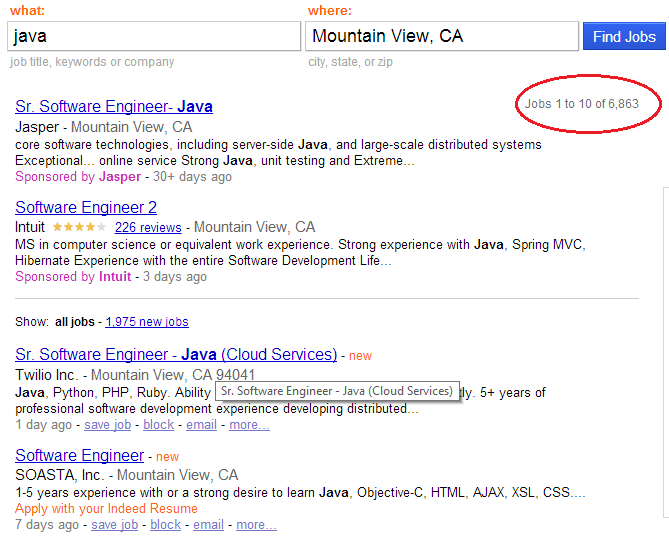
\includegraphics[scale=0.6]{images/indeed1.png}
  \caption{Search result of Indeed}
  \label{fig:Indeed}
\end{figure}

The reason for such result is because current job searching web sites use the same information retrieval technology like ``Inverted index'' \cite{zobel2006inverted} as the common search engines, which just use keywords to map all the stored documents. Modern search engines all have some ranking algorithms to sort the searching result, like page rank \cite{page1999pagerank}, so the top results always be the most related ones. But such algorithms are unavailable to the job searching systems, because the criteria  of how to rank the job searching result is very personalized. A great job opening for one job seeker maybe looks not good to the other, because the goodness of a job to a specular job seeker is heavily depend on his personal background, like his education or professional experience etc.

Since the people's resumes contain the most important background information, we believe the content of the resume could be used to rank the job openings. We give an example of resumes in Table~\ref{tab:resume}. In this thesis we created a web system which could use the resumes of job seekers to find the jobs that match their profiles best. The main idea is to calculate the similarity between the resume model and job models, which should be generated from resumes and job descriptions. We want to transfer the job searching task from key word searching to candidate model matching. The matching result should be sorted by the matching score, higher matching score means a better matching. The matching algorithm does not only help job seekers to find the appreciate job opening, but also offer priority to them~\cite{gueutal2006brave}.  The job with higher matching score means the job is more appropriate to the job seeker, and if he applies the job, the chance of getting the interview will be higher as well. Figure~\ref{fig:Matching} shows how this approach works.


\begin{figure}[htbp]
  \centering
  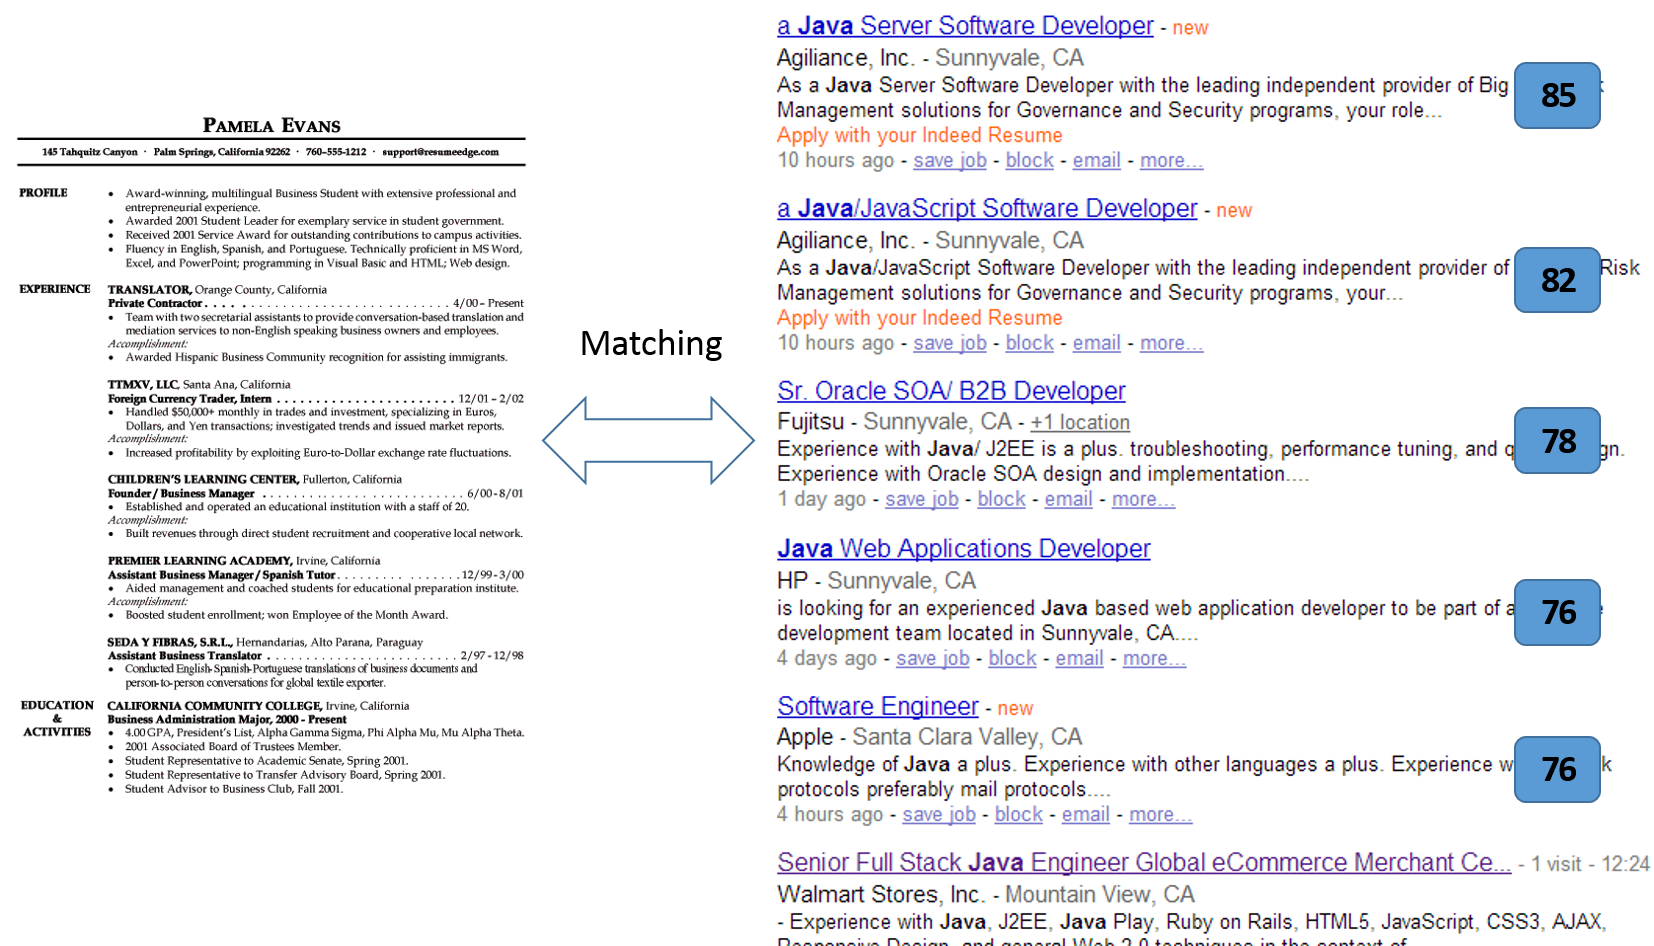
\includegraphics[scale=0.5]{images/matching.png}
  \caption{Matching the job opening with Resume}
  \label{fig:Matching}
\end{figure}


\begin{table}[!p]
 \small
\caption{Example of Resume} % title of Table
\centering % used for centering table
\begin{tabular}{    |  p{15cm} |  }
\hline
\begin{center}\normalsize{\textbf {Ryan Richman}}\\
\end{center}
\\
WORK EXPERIENCE\\
\\
\textbf{Web Developer}\\
Fabuso/Advanced Brain Technologies - Ogden, UT - February 2012 to Present \\
Created dynamic custom web applications for e-commerce and B2B clients. \\
Designed and edited audio-visual content for many different online applications. \\
Spearheaded migration of largest client's website from Joomla platform into Java code base. \\
Built dynamic event pages, document viewers, training course applications, shopping carts, and more. \\
Utilized advanced e-mail standards and best practices, SQL database queries, and Google Analytics.\\
\\
\textbf{IT Representative}\\
Advanced Brain Technologies - Ogden, UT - April 2011 to February 2012 \\
Provided internal software/hardware support for 20 employees both in-house and remote. \\
Designed using wireframes, tested, and debugged web pages. \\
Constructed dynamic projects and graphic designs in coordination with senior developers. \\
Created HTML-optimized emails for hundreds of campaigns. \\
Maintained and upgraded hardware for 20+ workstations company-wide. \\
\\
\textbf{Founder/Head Technician}\\
Teton Media Services, LLC - Ogden, UT - October 2008 to January 2011 \\
Created and developed websites for personal and small business customers \\
Sold high-speed cable and satellite internet access on the phone, online and in person. \\
Installed and serviced high-speed internet access hardware in residential and commercial properties. \\
Designed and implemented networking solutions for homes and businesses. \\
\\
 
\\
EDUCATION\\
\\
Computer Science \\
Weber State University - Ogden, UT 2010 to 2013 \\
\\
ADDITIONAL INFORMATION \\
\\
Technical Skills \\
Adept in the use of HTML, CSS, jQuery, Javascript, SQL, PHP, JSON, Windows, Windows Server, Mac, and Photoshop. \\

\\
\hline

\end{tabular}
\label{tab:resume} % is used to refer this table in the text
\end{table}


\section{Contribution}

We make the following contributions in this work:

\begin{enumerate}
    \item  We proposed a finite state transducer based matching tool to extract information from unstructured data source, which is a lightweight and flexible library, and can be extend in very easy ways.
    \item  We proposed a semi-automatic approach, which could collect technical terms from data sources, and by which we created a domain specific ontology for recruitment.
    \item  We proposed statistical-based ontology similarity measure, which can measure the similarities between technical terms .
    \item  We proposed a approach which combine the keyword searching and model matching to retrieval jobs.
\end{enumerate}

\section{Organizations}
The subsequent chapters are organized as follows: We first describe what has been done in terms of prior work.  We introduce some basic conception of recommender systems, and how to apply recommender technologies into Job Recommender Systems. Some previous Job Recommender Systems will be introduced,  their advantages and limits will be discussed as well.  Two import problems of content-based Job Recommender Systems, Information Extraction and Similarity Calculation, will be fully explained.

Then we introduce our work, JobFinder, a the Personalized Resume-Job Matching System. At first we give a overview of the system, which includes the architecture and the interfaces. Then we explained details of how we resolve the problems of information extraction and model similarity calculation. We proposed a finite state transducer library which can match patterns in sentence, and extracts related information. Ontology play an important role in this system. We will present how to construct the domain specific ontology for recruitment. We also give a brief review of different ontology similarity measures, and explain the statistical-based ontology similarity measure we used in this system.

Finally, we evaluate the accuracy of our information extraction approach. We used NDCG to evaluate the accuracy of statistical-based ontology similarity measure. To evaluate the performance of the system, we compared our algorithm to some classical information retrieval approaches by precision@k and NDCG. We created a data set job descriptions as documents, and use resumes as query to retrieval documents. The result shows the ranking performance is better than other information retrieval approaches.
